% Prof. Dr. Ausberto S. Castro Vera
% UENF - CCT - LCMAT - Curso de Ci\^{e}ncia da Computa\c{c}\~{a}o
% Campos, RJ,  2023
% Disciplina: Paradigmas de Linguagens de Programa\c{c}\~{a}o
%



\chapter{ Introdu\c{c}\~{a}o}

Se tornando uma das principais referencias quando se trata de diversas necessidades, a linguagem R é uma das mais populares atualmente.Na introdução deste livro, apresentaremos primeiramente um pouco da jornada dessa linguagem, com seus aspectos históricos. Além de suas principais áreas de aplicação, uma breve explicação sobre tais áreas e  alguns exemplos desses usos.

   \section{Aspectos hist\'{o}ricos da linguagem R}

Segundo \cite{Lander2017}, a história da Linguagem R remonta aos anos 70, com a criação da linguagem S, que serviu de base para a implementações de novos recursos.
A linguagem S, desenvolvida na AT\&T Bell Labs, primariamente pelo John Chambers, inventada a partir da necessidade de um sistema interativo de Analise Estatística, serve de fundamento para o surgimento da R, que por sua vez, foi produzida por conta de uma motivação parecida com de sua "antecessora", a busca por um melhor ambiente de software para Analise Estatística.A linguagem R então, surge nos anos 90, no Departamento de Estatística da Universidade de Auckland pelas mãos dos Estatísticos Ross Ihaka e Robert Gentleman.

Acostumados com o S, percebendo a necessidade de um melhor ambiente de Software e observando que não haviam softwares compatíveis no mercado, decidiram criar sua própria linguagem, nascendo assim a R.

De acordo com \cite{Cotton2013}, o fato da jornada dessa linguagem ter seu relativo começo desde os anos 70 se torna importante pois ela foi se desenvolvendo por décadas, não começou a partir do nada. Ela veio de algo e se tornou o que é hoje. 
Uma de suas principais características sendo a forma como se desenvolveu, tendo uma natureza de maior liberdade para contribuições, com seus usuários sendo capazes de, caso necessário, criarem seus próprios pacotes e compartilharem, R continua crescendo a partir de quem a usa.\cite{Chang2019}

%Algumas linguagens s\~{a}o consideradas  tradicionais (como mostrado na Fig.\ref{ling1}) e outras s\~{a}o consideradas modernas (ver Fig.\ref{ling2}). Devemos observar aqui, que a inclus\~{a}o de qualquer figura, significa que ela deve ser referenciada em algum lugar do texto
   \begin{figure}[H]
     \begin{center}
        \caption{Logos da Linguagem R} \label{ling1}
        
\includegraphics[width=12cm]{R01.png} \\
        {\tiny \sf Fonte: O autor deste trabalho }
     \end{center}
    \end{figure}
Seu nome, como mostrado na logo acima, provém das inicias dos seus criadores (Ross Ihaka e Robert Gentleman) e de um jogo figurado com a Linguagem S.

%Algumas figuras s\~{a}o criadas o elaboradas pelo mesmo autor, neste caso, deve-se escrever como fonte "O autor", "Os autores", etc. Figuras que incluam imagens de outras fontes deve-se especificar claramente, indicando o link o referencia correspondente, por exemplo, uma imagem que aparece em \cite[p. 93]{Sprankle2012}, \'{e} mostrada na Fig.\ref{afp} e a fonte deve ser indicada na parte inferior da figura.
 %  \begin{figure}[H]
  %  \begin{center}
   %     \caption{Algoritmo, Diagrama de fluxo, e Pseudo-c\'{o}digo} \label{afp}
    %    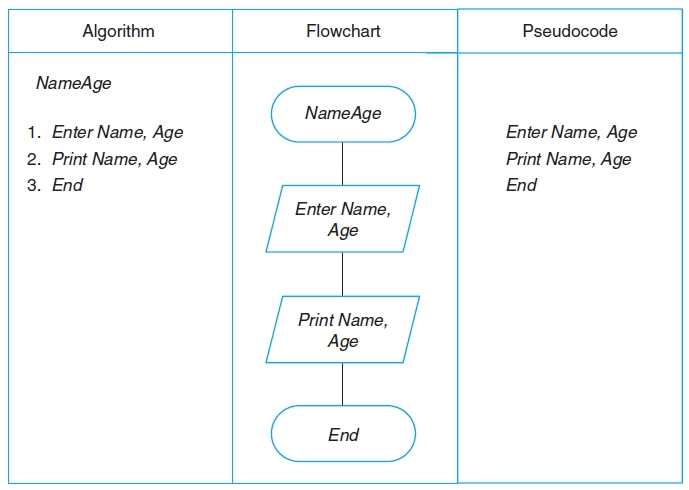
\includegraphics[width=10cm]{afp.jpg} \\
     %   {\tiny \sf Fonte: \cite[p. 93]{Sprankle2012} }
    %\end{center}
   %\end{figure}

   \section{\'{A}reas de Aplica\c{c}\~{a}o da Linguagem}
   A linguagem R, como dito, surge com a filosofia de ser uma ferramenta para a Analise de Dados em geral. Sendo útil e aplicada em diversas áreas relacionadas com essa ciência \cite{Wickham2016}. Tendo por exemplo: a Data Science, Big Data, Analise de Dados, Machine Learning, Estatística Computacional, entre outros. Além desses, a Linguagem R, sendo uma linguagem multi-paradigma, também suporta e é utilizada na Programação Orientada a Objetos. Veremos a seguir, alguns desses exemplos. 

        \subsection{ Data Science}
        Segundo \cite{SpiegelHalter2021} a Data Science, sendo uma das áreas da programação que mais cresce atualmente, abarca diversas necessidades e possibilidades. Tendo como objetivo criar, manipular e extrair o máximo possível de conhecimento a partir de dados para então gerar valor e melhorar processos, produtos e serviços, requer de seu profissional habilidades em diferentes campos, incluindo estatística, matemática, programação, visualização de dados entre outros.
        
        De acordo com \cite{Kabacoff2015}, cresce cada vez mais a quantidade de dados e informações com as quais empresas devem lidar para terem seu desempenho e custo otimizados, e se torna necessária a utilização de outras tecnologias mais eficientes para tratar dessa área. R surge então como uma das principais opções para esses desafios, tendo sida desenvolvida justamente para análise de dados e visualização desses resultados.  
        
        Por ser um software open-source, conta com uma massiva comunidade de usuários e desenvolvedores, o que garante uma evolução constante da linguagem e de suas utilidades. Essa sendo uma de suas maiores vantagens, possui milhares de pacotes à disposição de qualquer um para qualquer finalidade. Alguns desses se tornando referências para objetivos específicos, nos baseando no \cite{Wickham2016} achamos, por exemplo: ggplot2 para a visualização de dados, data.table para a manipulação de dados, entre outros.
        
        Embora um cientista de dados necessite de especialização em diversas áreas de conhecimento, desde matemática até a programação em si, é bem amparado pela linguagem R e sua comunidade que constantemente cresce e facilita seus processos.

        \subsection{ Orienta\c{c}\~{a}o a objetos}
        Um dos paradigmas da linguagem de programação mais atuais é a Programação Orientada a Objetos (POO), se baseando em objetos, que podem ser entendidos como instâncias de classes, contendo atributos e métodos relacionados. Esse paradigma busca encapsular objetos, permitindo maior independência das suas operações. Com outros conceitos fundamentais, a POO busca tornar o código mais flexível e adaptável. \cite{Deitel2018}
        
        Embora muitos algoritmos de análise de dados e estatística não sejam implementados utilizando a Programação Orientada a Objetos, o uso esse paradigma pode ser benéfico quanto à organização do código em módulos reutilizáveis, facilitando a manipulação dos dados. Sendo comum usar objetos para representar conjuntos de dados, e métodos para ser possível acessar e manipular esses dados, como adicionar ou remover colunas ou calcular estatísticas referentes a esses conjuntos.
        
        Podemos encontrar então a utilização do POO em R no \cite{Mailund2017}. A linguagem sendo uma das principais da área, além de multi-paradigma, também utiliza esse paradigma, da forma citada acima, utilizando objetos para encapsular dados, ou também na construção de modelos estatísticos, por exemplo. 
        
        R trabalha com três diferentes sistemas de Orientação a Objetos: S3, S4 e RC. S3 sendo o mais simples sistema de classes, trabalha com poucas restrições e não tendo uma estrutura definida formalmente, tendo como ideia que existam funções genéricas para serem utilizadas como os métodos, de acordo com a classe do objeto. S4 é uma evolução do anterior, tendo uma estrutura mais formal e definida, permitindo uma maior especificação dos seus métodos e atributos.Já o RC, ou Reference Class, já é uma abordagem avançada de Orientação a Objetos, permitindo a criação de classes utilizando todos seus fundamentos, como a herança, polimorfismo e encapsulamento.

        \subsection{ outras} 
        Apesar de amplamente utilizada na Data Science e na POO, a linguagem R embarca diversas outras áreas, como por exemplo a área de Estatística Computacional, possuindo um vasto número de pacotes referentes a esse assunto, é uma das principais opções para estatísticos. Com grande capacidade para a analise de dados e modelagem estatística, se torna um destaque pra quem busca novas ferramentas.
        
        Outra área em que a linguagem R tem sido utilizada é a Machine Learning, R possui um ampla gama de pacotes voltados para a área do aprendizado de máquina, como regressão linear e logística, clusterização e outros também para análise preditiva. Com o foco na automação através de algoritmos, é um assunto bem amparado pelos pacotes desenvolvidos em R.
        